\section{High-level Design} \label{sec:peregrine-design}

\begin{figure}[t]
\centering
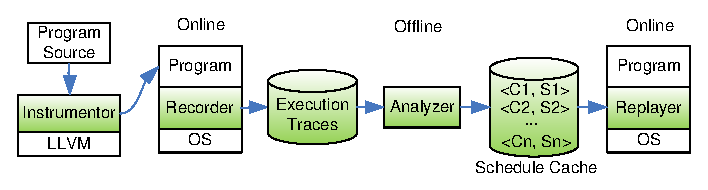
\includegraphics[width=.7\columnwidth]{peregrine/figures/overview.eps}
\caption{{\em \peregrine Architecture: components and data structures are
    shaded (and in green).}}\label{fig:peregrine-arch}
\end{figure}


Figure~\ref{fig:peregrine-arch} shows the architecture of \peregrine.  It has four main
components: the instrumentor, recorder, analyzer, and
replayer.  The \emph{instrumentor} is an LLVM~\cite{llvm} compiler plugin
that prepares a program for use with \peregrine.  It instruments synchronization
operations such as \vv{pthread\_mutex\_lock()}, which the recorder and
replayer control at runtime.  It marks the \vv{main()} arguments, data read
from \vv{read()}, \vv{fscanf()}, and \vv{recv()}, and values
returned by \vv{random()}-variants as
inputs.  We chose LLVM~\cite{llvm} as our instrumentation framework for
its compatibility with GCC and easy-to-analyze intermediate representation
(IR).  However, our approach is general and should apply beyond LLVM.
For clarity, we will present our examples and algorithms at the
source level, instead of the LLVM IR level.

The \emph{recorder} is similar to existing systems that deterministically
record executions~\cite{scribe:sigmetrics10,idna:vee06,smp-revirt:vee08}.
Our current recorder is implemented as an LLVM interpreter.  When a
program runs, the recorder saves the LLVM instructions interpreted for
each thread into a central log file.  The recorder does not record
external input data, such as data read from a file, because our
analysis does not need this information.  To schedule synchronization
operations issued by different threads, the recorder can use a variety of
DMT algorithms~\cite{cui:tern:osdi10}.  


\begin{figure}
\centering
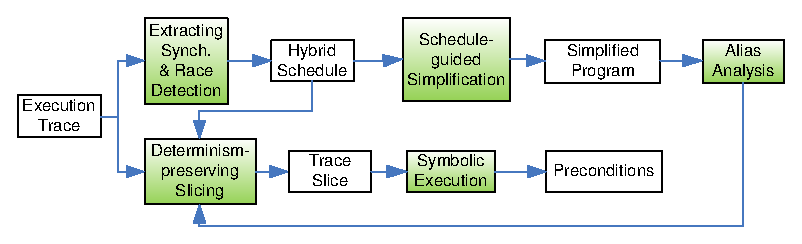
\includegraphics[width=0.7\columnwidth]{peregrine/figures/analyzer.eps}
\caption{{\em Analyses performed by the analyzer.}}\label{fig:peregrine-analyzer}
\end{figure}

The \emph{analyzer} is a stand-alone program that computes (1) a hybrid
schedule $S$ and (2) the preconditions $C$ required for reusing the schedule on
future inputs.  It does so using a series of analyses, shown in
Figure~\ref{fig:peregrine-analyzer}.  To compute a hybrid schedule, the analyzer
first extracts a total order of synchronization operations from the
execution trace.  It then detects data races according to this
synchronization order, and computes additional \emph{execution order} constraints
to deterministically resolve the detected races.
To compute the preconditions of a schedule, the analyzer first
\emph{simplifies} the program according to the schedule, so that alias
analysis can compute more precise results.  
It then slices the execution trace into a trace slice with instructions
required to avoid new races and reach all events in the schedule.  It
then uses \emph{symbolic execution}~\cite{symbolic-execution} to
collect preconditions from the input-dependent branches in the slice.
The trace slice is typically much smaller than the execution trace, so
that the analyzer can compute relaxed preconditions, allowing frequent
reuses of the schedule.  The analyzer finally stores $\langle C, S
\rangle$ into the schedule cache, which conceptually holds a set of such
tuples. (The actual representation is tree-based for fast
lookup~\cite{cui:tern:osdi10}.)



The \emph{replayer} is a lightweight user-space scheduler for reusing
schedules.  When an input arrives, it searches the schedule cache for a
$\langle C, S \rangle$ tuple such that the input satisfies the
preconditions $C$.  If it finds such a tuple, it simply runs the program
enforcing schedule $S$ efficiently and deterministically.  Otherwise,
it forwards the input to the recorder.
%  to record an execution and compute a new $\langle C, S \rangle$ tuple.

In the remainder of this section, we first use an example to illustrate
how \peregrine works, highlighting the operation of the analyzer
(\S\ref{sec:peregrine-example}).  We then describe \peregrine's deployment and usage
scenarios (\S\ref{sec:peregrine-deploy}) and assumptions (\S\ref{sec:peregrine-limitations}).

\subsection{An Example} \label{sec:peregrine-example}

%% \begin{figure}[t]
%% %\centering
%% \hspace{-.25in}
%% \begin{minipage}[t]{.525\textwidth}
%% \centering
%% 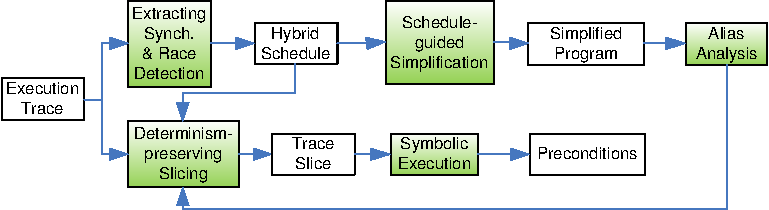
\includegraphics[width=\textwidth]{figures/analyzer}
%% \end{minipage}
%% \caption{{\em Analysis performed by the analyzer.}}\label{fig:analyzer}
%% \end{figure}

\begin{figure}[!ht]
\centering
\begin{minipage}{.5\textwidth}
\tiny \lgrindfile{peregrine/code/example.cpp.tex}
\end{minipage}
\caption{{\em Running example.} It uses the common
  divide-and-conquer idiom to split work among multiple threads.
  It contains write-write (lines L8 and L15)
  and read-write (lines L9 and L15) races on \vv{result} because
  of missing \vv{pthread\_join()}.} \label{fig:peregrine-example}
\end{figure}

Figure~\ref{fig:peregrine-example} shows our running example, a simple multithreaded
program based on the real ones used in our evaluation.  It first parses
the command line arguments into \vv{nthread} (line L1) and \vv{size} (L2),
then spawns \vv{nthread} threads including the main thread (L4--L5) and
processes \vv{size/nthread} bytes of data in each thread.  The thread
function \vv{worker()} allocates a local buffer (L10), reads data from a
file (L11), processes the data (L12--L13), and sums the results into
the shared variable \vv{result} (L14--L16).  The \vv{main()} function may
further update \vv{result} depending on \vv{argv[3]} (L7--L8), and finally
prints out \vv{result} (L9).  This example has read-write and write-write
races on \vv{result} due to missing \vv{pthread\_join()}.  This error
pattern matches some of the real errors in the evaluated programs such as
\pbzip.

\para{Instrumentor.} To run this
program with \peregrine, we first compile it into LLVM IR and instrument it with
the instrumentor.  The instrumentor replaces the synchronization
operations (lines L5, L14, and L16) with \peregrine-provided wrappers controlled by
the recorder and replayer at runtime.  It also inserts code to mark 
the contents of \vv{argv[i]} and the data from \vv{read()} (line L11) as
input.

\begin{figure}[!ht]
\begin{minipage}[t]{\columnwidth}
\centering
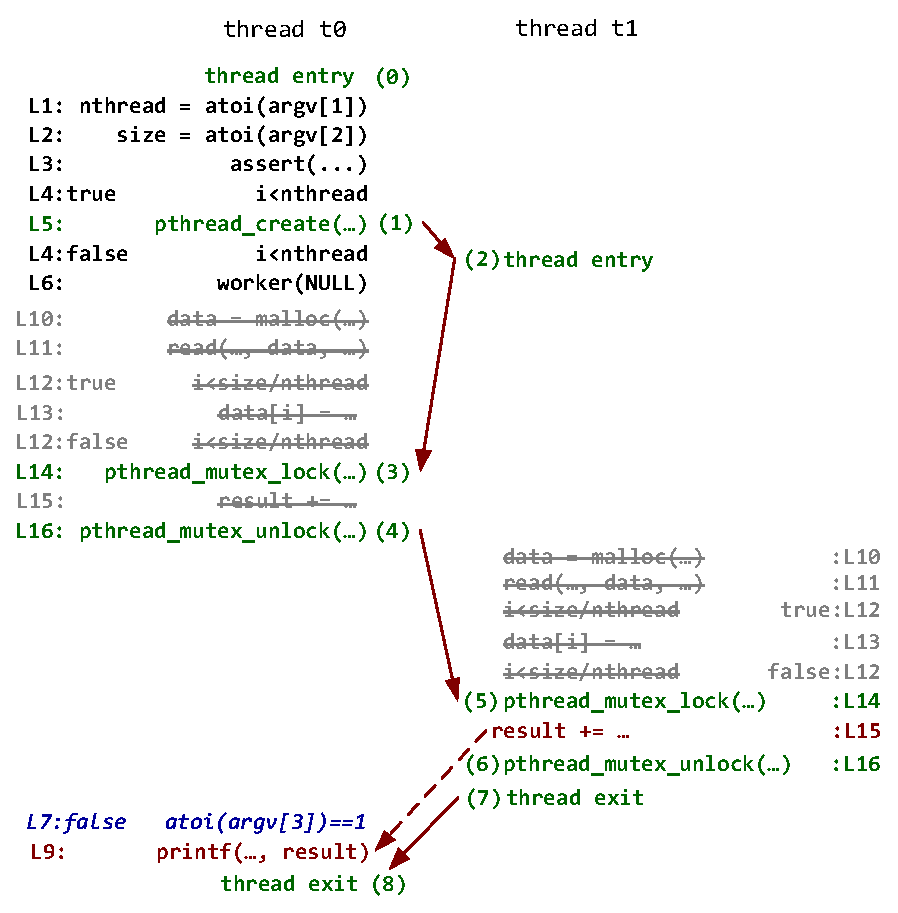
\includegraphics[width=0.7\textwidth]{peregrine/figures/trace}
\end{minipage}
\caption{{\em Execution trace, hybrid schedule, and trace slice.}  An
  execution trace of the program in Figure~\ref{fig:peregrine-example} on arguments
  ``\vv{2 2 0}'' is shown.  Each executed instruction is tagged
  with its static line number L$i$.  Branch instructions are also tagged
  with their outcome (true or false).  Synchronization operations (green),
  including thread entry and exit, are tagged
  with their relative positions in the synchronization order.  They form a
  sync-schedule whose order constraints are shown with solid arrows.  L15 of
  thread $t_1$ and L9 of thread $t_0$ race on \vv{result}, and this race is
  deterministically resolved by enforcing an execution order constraint
  shown by the dotted arrow.  Together, these order constraints form a hybrid
  schedule.  Instruction L7 of $t_0$ (italic and blue) is included in the
  trace slice to avoid new races, while L6, L4:false, L4:true, L3, L2, and
  L1 of $t_0$ are included due to intra-thread
  dependencies. Crossed-out (gray) instructions are elided from the
  slice.}\label{fig:peregrine-trace}
\end{figure}

\para{Recorder: execution trace.}
When we run the instrumented program with arguments ``\vv{2 2 0}'' to spawn
two threads and process two bytes of data, suppose that the recorder records
the execution trace in Figure~\ref{fig:peregrine-trace}.  (This figure also shows
the hybrid schedule and preconditions \peregrine computes, explained
later in this subsection.)  This trace is just one
possible trace depending on the scheduling algorithm the recorder uses.

\para{Analyzer: hybrid schedule.}
Given the execution trace, the analyzer starts by computing a hybrid
schedule.  It first extracts a sync-schedule consisting of the operations
tagged with (1), (2), ..., (8) in Figure~\ref{fig:peregrine-trace}.  It then detects races in
the trace according to this sync-schedule, and finds the race on
\vv{result} between L15 of thread $t_1$ and L9 of $t_0$.  It then computes an
execution order constraint to deterministically resolve this race, shown
as the dotted arrow in Figure~\ref{fig:peregrine-trace}.  The sync-schedule and
execution order constraint together form the hybrid schedule.  Although
this hybrid schedule constrains the order of synchronization and the last
two accesses to \vv{result}, it can still be efficiently reused because the
core computation done by \vv{worker} can still run in parallel.


\para{Analyzer: simplified program.}
To improve analysis precision, the analyzer simplifies the program according to the
hybrid schedule.  For instance, based on the number of
\vv{pthread\_create()} operations in the schedule, the analyzer
clones function \vv{worker()} to give each thread a copy,
so that the alias analysis separates different threads and determines that
the two instances of L13 in $t_0$ and $t_1$ access different
\vv{malloc}'ed locations and never race.

\para{Analyzer: trace slice.}
The analyzer uses
determinism-preserving slicing to reduce the execution trace into a trace
slice, so that it can compute relaxed preconditions.
The final trace slice consists of the instructions not crossed out
in Figure~\ref{fig:peregrine-trace}.
The analyzer computes this trace slice using inter-thread and 
intra-thread steps.  In the inter-thread step, it adds instructions
required to avoid new races into the slice.  Specifically, for $t_0$ it adds
the false branch of L7, or L7:false, because if the true branch
is taken, a new race between L8 of $t_0$ and L15 of $t_1$ occurs.  It
ignores branches of line L12 because alias analysis already determines that L13 of
$t_0$ and L13 of $t_1$ never race.

In the intra-thread step, the analyzer adds instructions required 
to reach all instructions identified in the
inter-thread step (L7:false of $t_0$ in this example) and all events in
the hybrid schedule.  It does so by traversing the execution trace
backwards and tracking control- and data-dependencies.  In this example, it
removes L15, L13, L12, L11, and L10 because no instructions currently in
the trace slice depend on them.  It adds L6 because without this call, the
execution will not reach instructions L14 and L16 of thread $t_0$.  It adds
L4:false because if the true branch is taken, the execution of $t_0$ will
reach one more \vv{pthread\_create()}, instead of L14,
\vv{pthread\_mutex\_lock()}, of $t_0$.  It adds L4:true because this branch
is required to reach L5, the \vv{pthread\_create()} call.  It similarly
adds L3, L2, and L1 because later instructions in the trace slice
depend on them.


\para{Analyzer: preconditions.}
After slicing, all branches from L12 are gone.  The
analyzer joins the remaining branches together as the
preconditions, using a version of \klee~\cite{klee:osdi08} augmented with
thread support~\cite{cui:tern:osdi10}.  Specifically, the analyzer marks
input data as \emph{symbolic}, and then uses \klee to track how this symbolic
data is propagated and observed by the instructions in the trace slice.
(Our \peregrine prototype runs symbolic execution within the recorder for
simplicity; see \S\ref{sec:peregrine-record}.)
If a branch instruction inspects symbolic data and proceeds down the true
branch, the analyzer adds the precondition that the symbolic data makes
the branch condition true.  The analyzer uses symbolic
summaries~\cite{castro:bouncer} to succinctly generalize common library
functions.  For instance, it considers the return of \vv{atoi(arg)}
symbolic if \vv{arg} is symbolic.

\begin{figure}[t]
\centering
\begin{minipage}[t]{3.1in}
\begin{scriptsize}
$(atoi\_argv_1 = 2) \wedge (atoi\_argv_2 \geq atoi\_argv_1) \wedge
  (atoi\_argv_3 \neq 1) $
\end{scriptsize}
\end{minipage}
\caption{{\em Preconditions computed from the trace slice in
    Figure~\ref{fig:peregrine-trace}.}  Variable $atoi\_argv_i$ represents the
  return of \vv{atoi(arg[i])}.} \label{fig:peregrine-precond}
\end{figure}

Figure~\ref{fig:peregrine-precond} shows the preconditions the analyzer computes
from the trace slice in Figure~\ref{fig:peregrine-trace}.
These preconditions illustrate two key benefits of \peregrine.
First, they are sufficient to ensure deterministic reuses of the schedule.
Second, they only loosely constrain the data size ($atoi\_argv_2$) and do
not constrain the data contents (from \vv{read()}), allowing frequent
schedule-reuses.  The reason is that L10--L13 are all sliced out.
One way to leverage this benefit is to populate a
schedule cache with small workloads to reduce analysis time, and then
reuse the schedules on large workloads.

\para{Replayer.}
Suppose we run this program again on different arguments ``\vv{2 1000 8}.''
The replayer checks the new arguments against the preconditions in
Figure~\ref{fig:peregrine-precond} using \klee's constraint checker, and finds that these
arguments satisfy the preconditions, despite the much larger data size.  
It can therefore reuse the hybrid schedule in Figure~\ref{fig:peregrine-trace}
on this new input by enforcing
the same order of synchronization operations and accesses
to \vv{result}.


\subsection{Deployment and Usage Scenarios} \label{sec:peregrine-deploy}

\peregrine runs in user-space and requires no special hardware, presenting few
challenges for deployment.  To populate a schedule cache, a user can
record execution traces from real workloads;
or a developer can run (small) representative workloads
to pre-compute schedules before deployment.  \peregrine
efficiently makes the behaviors of multithreaded programs more repeatable,
even across a range of inputs.  We envision that users can use this repeatability in
at least four ways.

\para{Concurrency error avoidance.} \peregrine can reuse well-tested schedules
collected from the testing lab or the field, reducing the risk of running
into untested, buggy schedules.  
Currently \peregrine detects and avoids only data races.  However, combined with
the right error detectors, \peregrine can be easily extended to detect and
avoid other types of concurrency errors.

\para{Record and replay.} Existing deterministic record-replay systems
tend to incur high CPU and storage overhead (\eg, 15X
slowdown~\cite{idna:vee06} and 11.7 GB/day
storage~\cite{smp-revirt:vee08}).  A record-replay system on top of \peregrine
may drastically reduce this overhead: for inputs that hit the
schedule cache, we do not have to
log any schedule.

\para{Replication.}
To keep replicas of a multithreaded program consistent, a replication tool
often records the thread schedules at one replica and replays them at
others.  This technique is essentially \emph{online}
replay~\cite{respec:asplos10}.
It may thus incur high CPU, storage, and
bandwidth overhead.  With \peregrine, replicas can maintain a consistent
schedule cache.  If an input hits the schedule cache, all replicas will
automatically select the same deterministic schedule, incurring zero
bandwidth overhead.

\para{Schedule-diversification.}  Replication can tolerate
hardware or network failures, but the replicas may still run into the same
concurrency error because they all use the same schedules.  Fortunately,
many programs are already ``mostly-deterministic'' as they either compute
the same correct result or encounter heisenbugs.  We can thus run \peregrine to
deterministically diversify the schedules at different replicas (\eg,
using different scheduling algorithms or schedule caches) to tolerate
\emph{unknown} concurrency errors.

\para{Applications of individual techniques.} The individual ideas in \peregrine
can also benefit other research effort.  For instance, hybrid schedules
can make the sync-schedule approach deterministic without recording
executions, by coupling it with a sound static race detector.
Determinism-preserving slicing can (1) compute input filters to block bad
inputs~\cite{castro:bouncer} causing concurrency errors and (2) randomize
an input causing a concurrency error for use with anonymous bug
reporting~\cite{castro:bug-report-privacy}.  Schedule-guided
simplification can transparently improve the precision of many existing
static analyses: simply run them on the simplified programs.  This improved
precision may be leveraged to accurately detect errors or even
verify the correctness of a program according to a set of schedules.
Indeed, from a verification perspective, our simplification technique
helps \emph{verify} that executions reusing schedules have \emph{no}
new races.

